%% 
%% ACS project dissertation template. 
%% 
%% Currently designed for printing two-sided, but if you prefer to 
%% print single-sided just remove ",twoside,openright" from the 
%% \documentclass[] line below. 
%%
%%
%%   SMH, May 2010. 

\documentclass[a4paper,12pt,twoside,openright]{report}
\usepackage{graphicx}

%%
%% EDIT THE BELOW TO CUSTOMIZE
%%

\def\authorname{Martin Marinov\xspace}
\def\authorcollege{St Edmund's College\xspace}
\def\authoremail{mtm46@cam.ac.uk}
\def\dissertationtitle{Remote video eavesdropping using a software-defined radio platform}
\def\wordcount{??,???}


\usepackage{epsfig,graphicx,parskip,setspace,tabularx,xspace,epstopdf,amssymb} 
\graphicspath{ {./images/} }

%% START OF DOCUMENT
\begin{document}


%% FRONTMATTER (TITLE PAGE, DECLARATION, ABSTRACT, ETC) 
\pagestyle{empty}
\singlespacing
% title page information
\begin{titlepage} 

\begin{center}
\noindent
\huge
\dissertationtitle \\
\vspace*{\stretch{1}}
\end{center}

\begin{center}
\noindent
\huge
\authorname \\
\Large
\authorcollege      \\[24pt]

\includegraphics{CUni3.eps}
\end{center}

\vspace{24pt} 

\begin{center}
\noindent
\large
{\it A dissertation submitted to the University of Cambridge \\ 
in partial fulfilment of the requirements for the degree of \\ 
Master of Philosophy in Advanced Computer Science} 
\vspace*{\stretch{1}}
\end{center}

\begin{center}
\noindent
University of Cambridge \\
Computer Laboratory     \\
William Gates Building  \\
15 JJ Thomson Avenue    \\
Cambridge CB3 0FD       \\
{\sc United Kingdom}    \\
\end{center}

\begin{center}
\noindent
Email: \authoremail \\
\end{center}

\begin{center}
\noindent
\today
\end{center}

\end{titlepage} 

\newpage
\vspace*{\fill}

\onehalfspacing
\newpage
{\Huge \bf Declaration}

\vspace{24pt} 

I \authorname of \authorcollege, being a candidate for the M.Phil in
Advanced Computer Science, hereby declare that this report and the
work described in it are my own work, unaided except as may be
specified below, and that the report does not contain material that
has already been used to any substantial extent for a comparable
purpose.

\vspace{24pt}
Total word count: \wordcount

\vspace{60pt}
\textbf{Signed}: 

\vspace{12pt}
\textbf{Date}:


\vfill

This dissertation is copyright \copyright 2014 \authorname. 
\\
All trademarks used in this dissertation are hereby acknowledged.



\newpage
\vspace*{\fill}

\singlespacing
\newpage
{\Huge \bf Abstract}
\vspace{24pt} 


This dissertation presents a software toolkit for remotely eavesdropping video monitors using a Software Defined Radio (SDR) receiver. It exploits compromising emanations from cables carrying video signals. Analogue video is usually transmitted one line of pixels at a time encoded as a varying current. This generates a wideband electromagnetic wave that can be picked up by an SDR receiver. The presented software can map the received field strength of each pixel to a grayscale value in order to show a real-time false colour estimate of the original video signal.

The software significantly lowers the costs required for undertaking a practical attack compared to existing solutions. Furthermore, it allows for an additional digital post-processing which can aid in analysing and improving the results. It also provides mobility for a potential adversary, requiring only a commodity laptop and an USB SDR dongle. The attacker does not need to have any prior knowledge about the victim's video display. All parameters such as resolution and refresh rate can be estimated with the aid of the software. 

The software comprises of a library written in C, a collection of plug-ins for various Software Define Radio (SDR) frontends and a Java based Graphical User Interface (GUI). It is designed to be a multi-platform application. All native libraries can be pre-compiled and packed into a single Java jar file which allows the toolkit to run on any supported operating system.

This report documents the digital processing techniques that have been employed in order to extract, detect and lock to a video signal. It also explains the architecture of the software system and the techniques used in order to achieve low latency and real-time interactivity. It demonstrates the usage of the system by performing a practical attack. It then gives some ideas about what could be improved further and some analysis of data that was collected during the development of the software.


\newpage
\vspace*{\fill}


\pagenumbering{roman}
\setcounter{page}{0}
\pagestyle{plain}
\tableofcontents
%% \listoffigures
%% \listoftables

\onehalfspacing

%% START OF MAIN TEXT 

\chapter{Introduction}
\pagenumbering{arabic} 
\setcounter{page}{1} 

\section{Related Work} 

[Related work and critique]

\section{Availability} 
[Github repo url]

\cite{kuhn2003compromising}

\chapter{Background}

\section{Electronic Emanations} 

\section{IQ sampling} 

\chapter{Methodology} 

\section{Analogue Video Signals}

Almost all contemporary video monitors are raster based. The image is transferred from the video controller to the display in scanlines that occur at a specific rate. Each of these scanlines contains a number of pixels which are continuously encoded as a time varying signal. This signal is generated internally in the video controller by an oscillator which runs at the pixel clock rate. The signal is thereafter multiplied by the pixel intensities at the specific time.

Let's assume that the signal started transmitting at time $t=0$, and each video frame contains $h$ scanlines, each of which contains $w$ pixels. The frequency with which frames are being generated is $f_{f}$ frames per second. Therefore the duration of transmission of each individual pixel is \begin{equation}
\label{eq:tdelta_definition}
T_{\Delta}=\frac{1}{w h f_{f}}
\end{equation}
Furthermore at time $t$ frame number $n_{t}$ started transmission where 
\begin{equation}
n_{t}=\lfloor t f_{f} \rfloor
\end{equation}
Therefore 
if we assume that the top left corner of a frame has coordinates $(0, 0)$, a pixel at position $(x, y)$ in frame $n_{t}$ will start to be transmitted at time
\begin{equation}
T_{(x,y)}= (y w + x + n_{t} w h) T_{\Delta}
\end{equation}
and will finish transmission before time 
\begin{equation}
T_{(x+1,y)} = T_{(x,y)} + T_{\Delta} =(y w + x + 1 + n_{t} w h) T_{\Delta}
\end{equation}
at which the next pixel will start transmitting.

In practice $w$ and $h$ are determined by the screen resolution and $f_{f}$ is simply the screen refresh rate. For a typical screen resolution of $width \times height$, it is true that $w \geq width$ and $h \geq height$. The reason is that video signals tend to have additional blanking intervals. This means more pixels are transmitted than what is in the active video region. This gives opportunity for the receiving monitor to synchronise its internal clock, calibrate its colour levels or in case of CRT, allow enough time for the electron beam to return to the beginning of the next line on the screen. The synchronisation timings for personal computers have been standardised by Video Electronics Standards Association (VESA) \cite{vesa}.

In order to decode an individual pixel, the receiving monitor has its own internal oscillator. It locks it to the pixel rate of the incoming signal either via an external clock source or using the blanking intervals. Once it receives the signal for an individual pixel, its amplitude (or binary content in case of digital signal) will correspond to the intensity. This allows the monitor to display the video in real time. If multiple colours are desired, they can be transmitted separately on different wires in the same fashion.

\section{Generated Radio Wave}

Let's assume the discrete pixels in a video signal have intensities $v_{i} (i \in \mathbb{Z})$ and are being transmitted for a duration of $T_{\Delta}=\frac{1}{w h f_{f}}$ (from \ref{eq:tdelta_definition}). Let's also assume that the shape of the pixel is $p(t)$ where $p(t)=0$ for $|t| > \frac{T_{\Delta}}{2}$. We know that pixel $i$ starts transmitting at time $t_{i}=i T_{\Delta}$ (if we assume that that pixel 0 was transmitted at $t=0$). Also the amplitude of the signal of the transmitted pixel is linearly dependant on its intensity $v_{i}$. Then the resulting signal between time $t_{i}$ and $t_{i+1}$ will have the form $v_{i} p(t-i T_{\Delta})$. To generalise for all $i$, the resulting actual transmitted radio wave in the time domain will have the form 
\begin{equation}
\label{eq:video_signal}
v(t) = \sum\limits_{i=-\infty}^{\infty} v_{i} p(t-i T_{\Delta})
\end{equation}
Which is a continuous function. Equation \ref{eq:video_signal} can be rewritten as a convolution with a Dirac delta function
\begin{equation}
\label{eq:vasconv}
v(t) = p(t) \ast \left( \sum\limits_{i=-\infty}^{\infty} v_{i} \cdot \delta(t-i T_{\Delta}) \right) = p(t) \ast \hat{v}(t)
\end{equation}
Where we have put
\begin{equation}
\label{eq:vhattdef}
\hat{v}(t) = \sum\limits_{i=-\infty}^{\infty} v_{i} \cdot \delta(t-i T_{\Delta})
\end{equation}
Note that this results in infinitesimally short (in time) spikes at values exact integer multiples of $T_{\Delta}$ with amplitudes corresponding to the pixel intensities at that time. We can view \ref{eq:vasconv} as the pixel shape being repeated at intervals of $T_{\Delta}$ modulated by $v_{i}$. We can also notice that $t$ can only take discrete values, namely  $i T_{\Delta}$, therefore we can write $i$ as $i = \lfloor \frac{t}{T_{\Delta}} \rfloor$ and therefore rewrite \ref{eq:vhattdef} as
\begin{equation}
\hat{v}(t) = \sum\limits_{i=-\infty}^{\infty} v_{ \lfloor \frac{t}{T_{\Delta}} \rfloor } \cdot \delta(t-i T_{\Delta}) = v_{ \lfloor \frac{t}{T_{\Delta}} \rfloor } \sum\limits_{i=-\infty}^{\infty} \delta(t-i T_{\Delta})
\end{equation}
Now let's revise some mathematical identities. According to the convolution theorem
\begin{equation}
\mathcal{F} \left\{ g \cdot h \right\} = \mathcal{F} \left\{ g \right\} \ast  \mathcal{F} \left\{ h \right\}
\end{equation}
Which reads: the Fourier transform of a multiplication of two functions is equivalent to the Fourier transforms of the individual functions convolved together. And vice versa
\begin{equation}
\mathcal{F} \left\{ g \ast h \right\} = \mathcal{F} \left\{ g \right\} \cdot  \mathcal{F} \left\{ h \right\}
\end{equation}
The convolution of the Fourier transform of two functions is equivalent to the individual Fourier transforms of the two functions multiplied together.
Also
\begin{equation}
\mathcal{F} \left\{ \sum\limits_{n=-\infty}^{\infty}  \delta(t-n k) \right\} = \frac{1}{k} \sum\limits_{n=-\infty}^{\infty}  \delta \left( t-\frac{n}{k} \right)
\end{equation}
Using the last three identities, we can write the Fourier transform of \ref{eq:vasconv} as
\begin{equation} 
\mathcal{F} \left\{ p(t) \ast \hat{v}(t) \right\} = V(f) =
\left[ \frac{1}{T_{\Delta}} \cdot P(f) \cdot \mathcal{F} \left\{ v_{ \lfloor \frac{t}{T_{\Delta}} \rfloor } \right\} \right] \ast
\left[ \sum\limits_{i=-\infty}^{\infty}  \delta \left( t-\frac{i}{T_{\Delta}} \right) \right]
\end{equation}
Where $P(f)$ is the Fourier transform of $p(t)$ and $V(f)$ is the Fourier transform of $v(t)$. If we put 
\begin{equation} 
G(f) = \frac{1}{T_{\Delta}} \cdot P(f) \cdot \mathcal{F} \left\{ v_{ \lfloor \frac{t}{T_{\Delta}} \rfloor } \right\}
\end{equation}
Then we we can arrive to our final conclusion that
\begin{equation}
V(f) = G(f) \ast
\left[ \sum\limits_{i=-\infty}^{\infty}  \delta \left( t-\frac{i}{T_{\Delta}} \right) \right]
\end{equation}
This simply means that the signal spectrum $G(f)$ repeats at regular intervals throughout the radio spectrum with a frequency of $\frac{1}{T_{\Delta}} = w h f_(f)$. Therefore we should expect to be able to tune our receivers at an integer multiple of that frequency and pick up the entire transmitted video signal (given that $G(f)$ is band limited and the bandwidth of our receiver is higher than the bandwidth of $G(f)$).

\section{Sampling Rate}

The Fourier transform of such a signal will therefore range from $\frac{-\nu_{max}}{2}$ to $\frac{\nu_{max}}{2}$ (all other elements will be zero). The lowest frequency components will be centred around DC while the highest one will span up to $\frac{\nu_{max}}{2}$ in each direction. Therefore in order to fully reconstruct the signal, we will need to sample an output from an antenna with a rate of $\nu_{max}$. However, the video cables are usually much shorter than those wavelengths and therefore they don't emit efficiently in this range. 

[Discuss how IQ relates to AM and how it can be used to reconstruct video.]

[Explain how the whole system works in high level]

[TODO! Explain how resolution and framerate detection works]

[Digital video]

\section{Sampling Rate}

[TODO! Explain how bandwidth relates to resolution width * height * framerate = samplerate ]

The sampling rate

\begin{figure}[h!]
\minipage{0.49\textwidth}
  \centering
    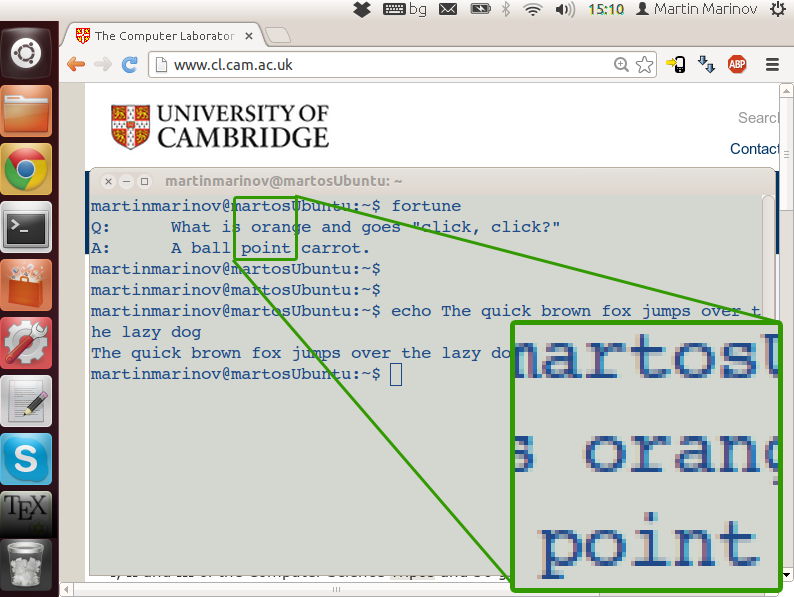
\includegraphics[width=0.5\textwidth]{sr_original}
  \caption{Transmitted image}
\endminipage\hfill
\minipage{0.49\textwidth}
  \centering
    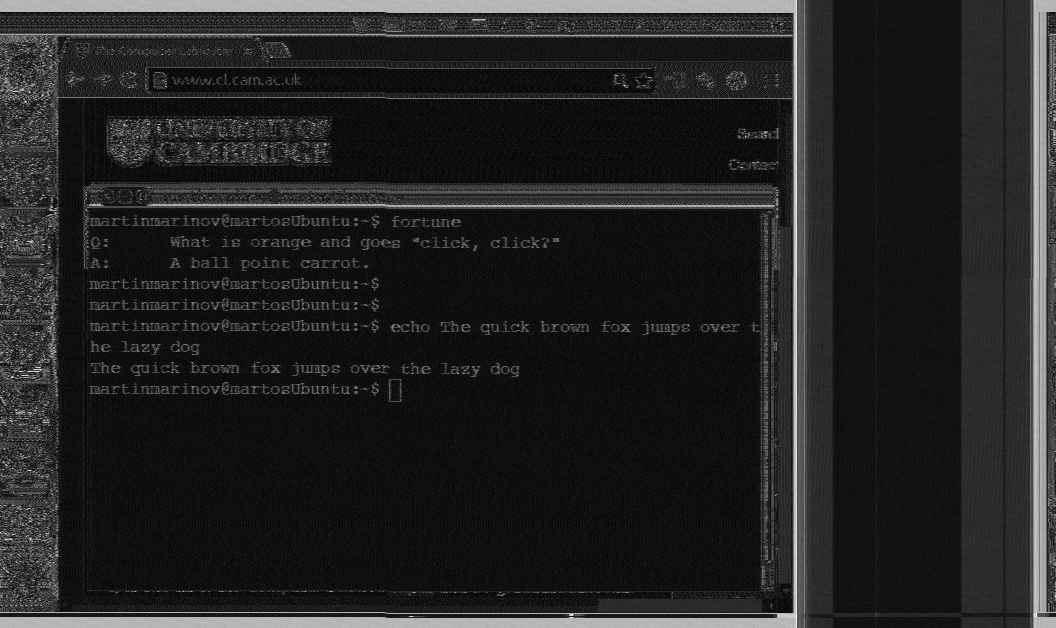
\includegraphics[width=\linewidth]{sr_50MHz_at_190MHz}
  \caption{50 MHz}
\endminipage\hfill
\minipage{0.49\textwidth}
  \centering
    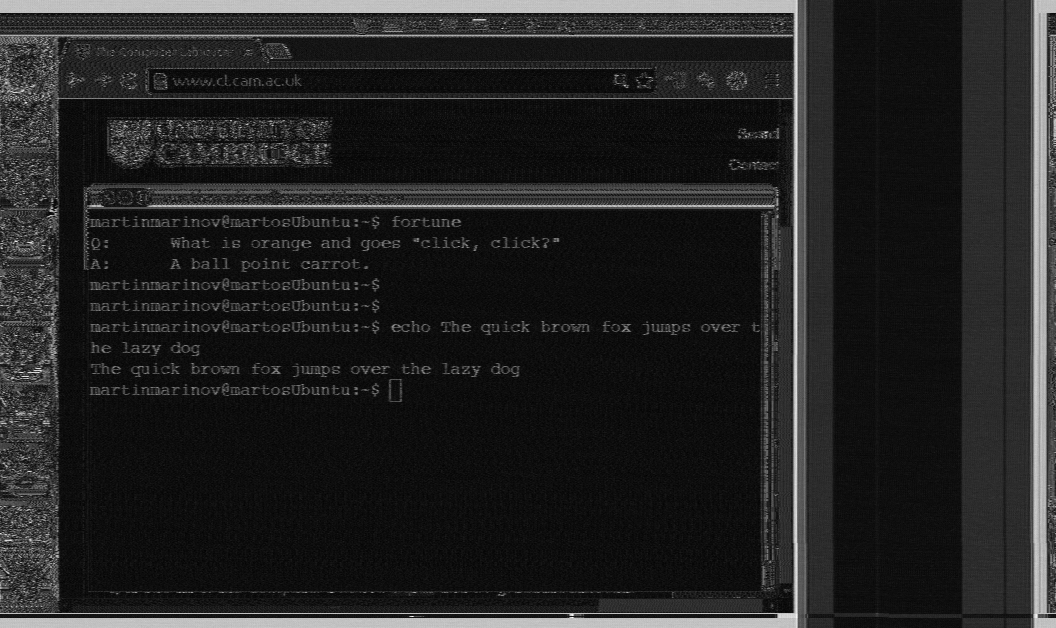
\includegraphics[width=\linewidth]{sr_40MHz_at_190MHz}
  \caption{40 MHz}
\endminipage\hfill
\minipage{0.49\textwidth}
  \centering
    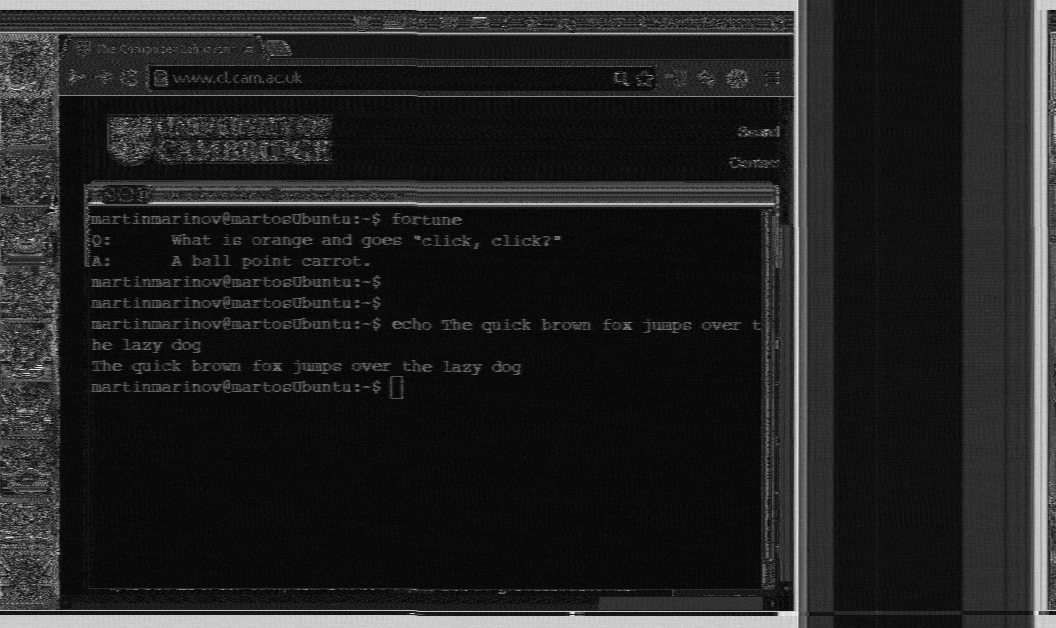
\includegraphics[width=\linewidth]{sr_30MHz_at_190MHz}
  \caption{30 MHz}
\endminipage\hfill
\minipage{0.49\textwidth}
  \centering
    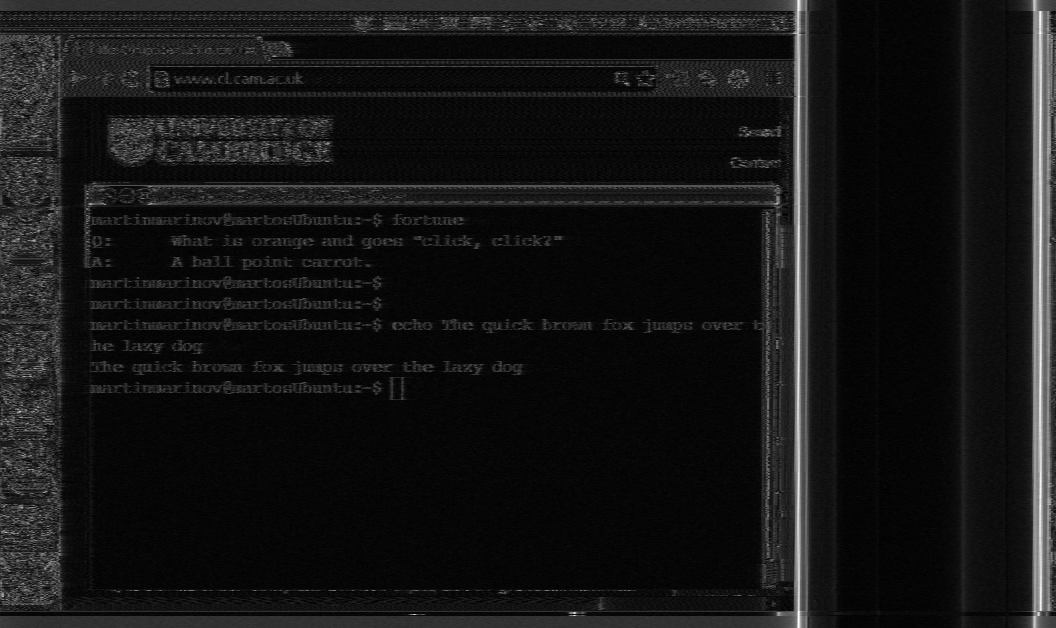
\includegraphics[width=\linewidth]{sr_20MHz_at_190MHz}
  \caption{20 MHz}
\endminipage\hfill
\minipage{0.49\textwidth}
  \centering
    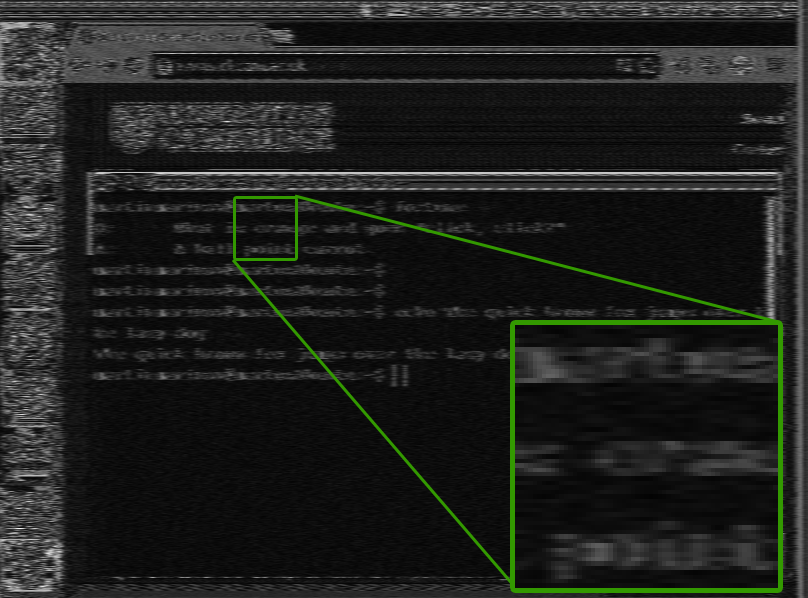
\includegraphics[width=\linewidth]{sr_10MHz_at_190MHz}
  \caption{10 MHz}
\endminipage\hfill
\minipage{0.49\textwidth}
  \centering
    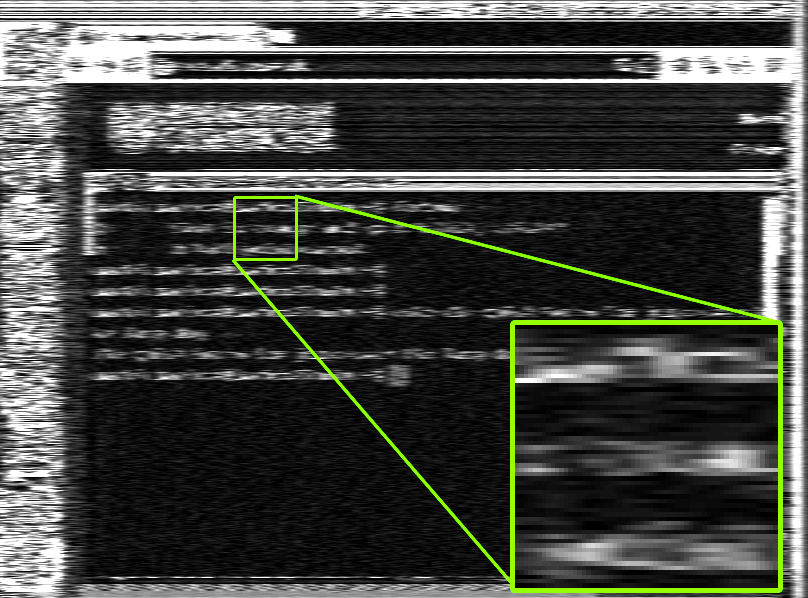
\includegraphics[width=\linewidth]{sr_5MHz_at_190MHz}
  \caption{5 MHz}
\endminipage
\end{figure}


\chapter{Practical attack} 

Before explaining how the software works internally, let's present a demonstration of a practical video eavesdropping attack. Its main aim is to show the ease with which such an attack could happen. In the meantime this will give an opportunity to explain the characteristics of the received signal and how they are exploited.

As in the real world, we will start with no knowledge of the victim's system. We will estimate the frequency at which the emission strength has the best Signal to Noise Ratio (SNR). We will then analyse the signal to detect the resolution and refresh rate of the screen. We will afterwards lock onto the signal and try to recover the original video. We will also discuss some techniques that could be utilized to improve the quality of the image.

\section{The Setup}

The choice for a SDR front-end for this demonstration is a USRP B200\footnote{Refer to \ref{sec:hw} Hardware for discussion on currently available SDR devices.}. Depending on the particular requirements, an attacker might prefer mobility over accuracy and choose the smaller Mirics FlexiTV\texttrademark MSi3101 SDR USB Dongle. However, for this demonstration we will attempt to obtain the highest possible resolution. Therefore we need an SDR radio that is capable of obtaining a wide bandwidth. This makes the 32 MHz of Bandwidth that the USRP provides a much better choice than the 8 MHz available from the Mirics dongle.

[Antenna]

[Location of victim]

[Victim's fonts]

\section{Preparation}

\chapter{Implementation} 

\section{Hardware}
\label{sec:hw} 

\begin{figure}[h!]
 
  \centering
    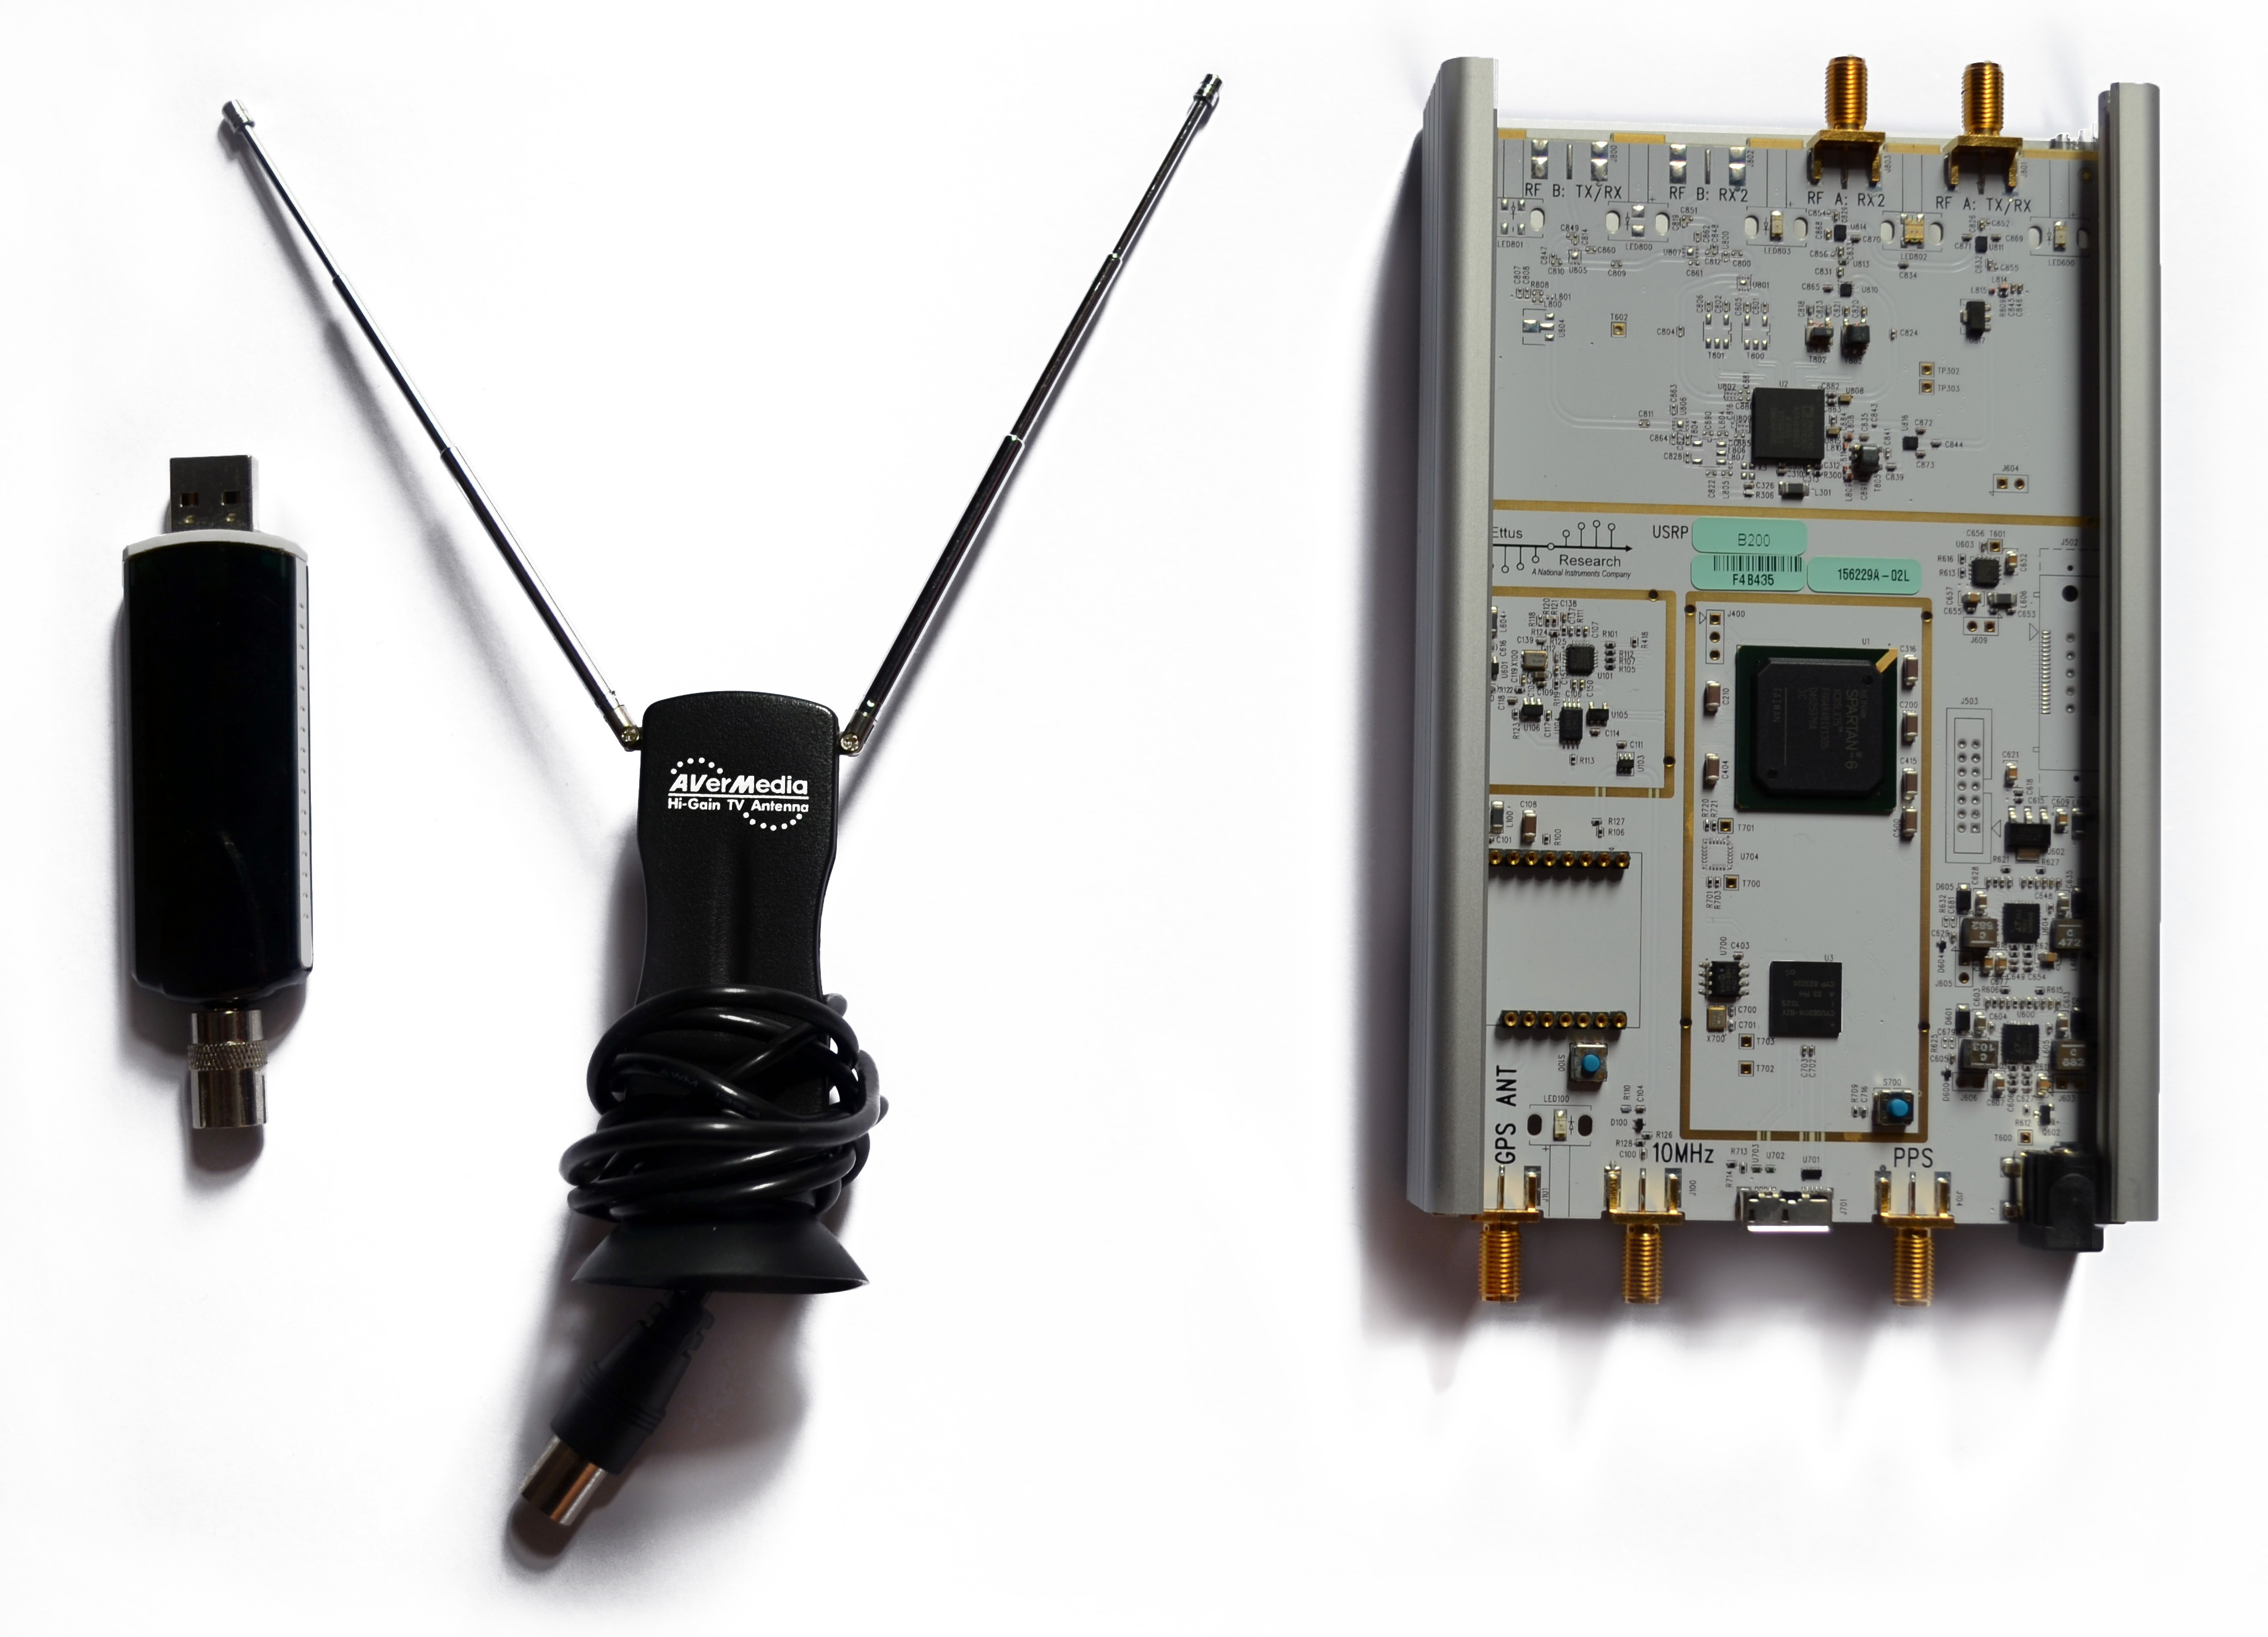
\includegraphics[width=0.9\textwidth]{equipment}
    \caption{From left to right: MSi3101, AverMedia antenna and USRP B200}
\end{figure}


\section{Architecture}

\subsection{Main Library}

\subsection{JavaGUI}

\subsubsection{Multiplatform}

\subsubsection{Graphical Interface}

\subsubsection{Visualisation}

\section{Digital Signal Processing}

\subsection{Overview}

\subsection{Signal Reconstruction}

\subsubsection{Multithreading}

\subsubsection{Demodulation}

\subsubsection{Re-sampling}

\subsubsection{Auto Gain}

\subsubsection{Low-pass}

\subsection{Frame Synchronization}

\subsection{Resolution Detection}

\subsection{Extended Bandwidth}

\subsection{Testing and Benchmarking}

\chapter{Summary and Conclusions} 

[Summarize results]

[potential future work]

\appendix
\singlespacing

\bibliographystyle{unsrt} 
\bibliography{dissertation} 

\end{document}
